\documentclass{sigcomm-alternate}
\pdfpagewidth=8.5in
\pdfpageheight=11in

% added by Vaibhav
%----------------------------------------------------------------------
\usepackage{cite}
\usepackage[utf8]{inputenc}
\usepackage[table]{xcolor}
\usepackage[T1]{fontenc}
\usepackage[nolist]{acronym}
\usepackage{url}
\usepackage{todonotes}
\usepackage{booktabs}
\usepackage{listings}
\usepackage[font=footnotesize,caption=false]{subfig}
\usepackage[multiple]{footmisc}
\usepackage{color,soul}
\usepackage{amsfonts}
\usepackage{epigraph}
\usepackage[colorlinks=true,allcolors=blue]{hyperref}

\definecolor{gray}{gray}{0.93}
%----------------------------------------------------------------------

\begin{acronym}
  \acro{LMAP}{Large-Scale Measurement of Broadband Performance}
  \acro{FCC}{Federal Communications Commission}
  \acro{IMC}{Internet Measurement Conference}
  \acro{CDN}{Content Delivery Network}
  \acro{CDH}{Cloudera Distribution Including Apache Hadoop}
  \acro{HDFS}{Hadoop Distributed File System}
  \acro{IoT}{Internet of Things}
  \acro{MAMI}{Measurement and Architecture for a Middleboxed Internet}
  \acro{FCC}{Federal Communications Commission}
  \acro{MBA}{Measuring Broadband America}
  \acro{COTS}{Commercial Off-the-shelf}
  \acro{IRR}{Internet Routing Registry}
  \acro{SDN}{Software-defined Network}
  \acro{QoE}{Quality of Experience}
  \acro{QoS}{Quality of Service}
  \acro{MA}{Measurement Agent}
  \acro{PTS}{Post and Telecom Authority}
  \acro{AS}{Autonomous Systems}
  \acro{DSL}{Domain Specific Language}
  \acro{mPlane}{Measurement Plane}
  \acro{QUIC}{Quick UDP Internet Connections}
  \acro{WebRTC}{Web Real-Time Communication}
  \acro{NFV}{Network Function Virtualization}
  \acro{Ark}{Archipelago}
  \acro{NAS}{Network-attached Storage}
\end{acronym}


\begin{document}

\title{Dagstuhl Perspectives Workshop on Global Measurements: Practice and
Experience}
\title{Global Measurements: Practice and Experience \\ (Report on Dagstuhl Seminar \#16012)}

\numberofauthors{1}
\author{
\begin{tabular*}{0.9\textwidth}%
{@{\extracolsep{\fill}}ccc}
Vaibhav Bajpai & Arthur W. Berger & Philip Eardley \\
\affaddr{Jacobs University} & \affaddr{Akamai Technologies} & \affaddr{British Telecom R\&D} \\
\affaddr{Bremen, DE} & \affaddr{Cambridge, US} & \affaddr{Ipswich, GB} \\
\email{v.bajpai@jacobs-university.de} & \email{awberger@csail.mit.edu} & \email{philip.eardley@bt.com}
\end{tabular*}\\
\begin{tabular}{c}
\end{tabular}\\
\begin{tabular*}{0.6\textwidth}%
{@{\extracolsep{\fill}}cc}
Jörg Ott & Jürgen Schönwälder \\
\affaddr{TU München} & \affaddr{Jacobs University} \\
\affaddr{München, DE} & \affaddr{Bremen, DE} \\
\email{ott@in.tum.de} & \email{j.schoenwaelder@jacobs-university.de}
\end{tabular*}\\
\begin{tabular}{c}
\end{tabular}\\
\begin{tabular}{c}
{\normalsize This article is an editorial note submitted to CCR. It has NOT
been peer reviewed.}\\
{\normalsize The authors take full responsibility for this article's
technical content. Comments can be posted through CCR Online.}
\end{tabular}
}

\maketitle

\begin{abstract}

This article summarises a 2.5 day long Dagstuhl seminar on Global
Measurements: Practice and Experience held in January 2016.  This seminar was
a followup of the seminar on Global Measurement Frameworks held in 2013, which
focused on the development of global Internet measurement platforms and
associated metrics.  The second seminar aimed at discussing the practical
experience gained with building these global Internet measurement platforms.
It brought together people who are actively involved in the design and
maintenance of global Internet measurement platforms and who do research on
the data delivered by such platforms. Researchers in this seminar have used
data derived from global Internet measurement platforms in order to manage
networks or services or as input for regulatory decisions. The entire set of
presentations delivered during the seminar is made publicly available at
\cite{dagstuhl-materials}.

\end{abstract}

% referrred: http://www.acm.org/about/class/ccs98-html
%\category{C.2.3}{Computer-Communication Networks}{Network Operations}[Network
%monitoring]

% referred: http://www.acm.org/sigs/publications/sigguide-v2.2sp
%\terms{Measurement, Performance}

\keywords{Internet measurements, Quality of experience, Network management,
Traffic engineering}

% sections
%----------------------------------------------------------------------
%**************************************************************************
\section{Introduction}\label{sec:introduction}
%**************************************************************************

%------------------------ Motivation

Several large-scale Internet measurement platforms have been deployed during
the last years in order to understand how the Internet is performing, to
observe how it is evolving, and to determine where failures or degradations
occur. Examples are the CAIDA \ac{Ark} platform \cite{kclaffy:ccr:2016} (used
for Internet topology discovery and detecting congestion on interdomain
links), the SamKnows platform \cite{vbajpai:comst:2015} (used by regulators
and network operators to study network performance), the RIPE Atlas platform
\cite{ripencc:ipj:2015, vbajpai:ccr:2015} (that provides measurement services
to network operators and researchers), the Netradar system
\cite{ssonntag:wiopt:2013} (for performing wireless performance measurements),
and the BISmark project \cite{ssundaresan:usenix:2014}.  European
collaborative research projects lately have been working on a \ac{mPlane}
\cite{btrammell:commag:2014} and how to incorporate measurement results into
network management systems (e.g., Leone) \cite{leone}. Related projects (e.g.,
Flamingo) \cite{flamingo} are increasingly working with measurement data from
these platforms.  Large-scale measurements are meanwhile also used to drive
network operations or to dynamically adjust how services are delivered to
customers. \ac{CDN} providers use measurement data to optimize content caches
and to tune load balancing algorithms. One key challenge is that global
Internet measurement systems can generate large amounts of data that need to
be processed to derive relevant information.

%------------------------ Goals

This seminar (\#16012) was a followup of the Dagstuhl seminar on Global
Measurement Frameworks (\#13472) \cite{peardley:dagstuhl:2013}. The main focus
of the first seminar was an exchange of ideas on the development of global
measurement infrastructures, frameworks and associated metrics. Some of this
work is now further pursued in standardization bodies
\cite{vbajpai:comst:2015}  such as the IETF \ac{LMAP} working group and the
Broadband Forum.  The goal of this followup seminar was to focus on the
experience obtained with different metrics, tools, and data analysis
techniques. It provided a forum for researchers to exchange their experience
with different practices to conduct global measurements. The aim was to
identify what works well in certain contexts, what has proven problematic in
other contexts, and identify open issues that need further research.

The seminar approached this by looking at three distinct dimensions: $a)$
Measurement metrics, $b)$ data processing technologies and $c)$ data analysis
methodologies. Some key questions were: $a)$ Which metrics have been found
useful for measuring \ac{QoE} of certain classes of services?  Which metrics
have been found problematic? Is it possible to find indicators for good
metrics and problematic metrics?, $b)$ Which technologies have been found
useful for storing and processing large amounts of measurement data?  Which
technologies were found to be problematic?  Are there new promising
technologies that may be used in the future? What are the specific
requirements for dealing with large-scale measurement data and how do they
relate to or differ from other big data applications? and $c)$ Which data
analysis techniques have been found to be useful? Which data analysis
techniques have been found to be problematic? Are there any novel promising
techniques that need further research and development?

Although at the seminar the participants chose to organize the discussions on
more general topics than these specific questions, during the discussions most
of these questions were addressed to one degree or another.

%**************************************************************************
\section{Invited Presentations}\label{sec:invited-presentations}
%**************************************************************************

The invited presentations were intended as a basis for triggering discussions
and identifying areas for group work.

% ------------ Henning Schulzrinne
\subsection{Experiences from Measuring Networks}

Henning Schulzrinne (Columbia University / FCC) began by sharing experiences
gained through five iterations of the \ac{FCC} \ac{MBA} program \cite{mba},
consisting of around 5,500 measurement hosts. The project is unique in that it
is a collaboration between a regulator, a contractor (SamKnows
\cite{vbajpai:comst:2015}) developing and managing the infrastructure, about a
dozen consumer ISPs and their trade associations, backbone ISPs, two
third-party measurement facilities (M-Lab \cite{cdovrolis:ccr:2010} and
Level3) and university collaborators.  Establishing a code of conduct and
setting up a (lightweight) collaborative structure early on has helped work
through conflicts and deal with data quality challenges. Since these
measurements are used by competing providers, e.g., in TV commercials, the
stakes are perceived to be higher than just scientific discovery. The project
emphasizes long-term comparability of measurements, open data and
reproducibility. For example, all scripts and spreadsheets used to produce the
annual report are made available.

He described how the measurement report has changed, increasingly emphasizing
variability in performance, across time and the user population, not just
averages.  One of the more contentious issues has been dealing with unexpected
soft and subtle failures of measurement infrastructure, e.g., memory leaks and
Ethernet port speed issues, as well as what to consider outliers. For example,
a time period was excluded from the measurement month used for reporting since
it coincided with the download traffic of iOS 8.0. Users may also delay
upgrading their cable modem, causing performance to drop below the offered
rate. In the long term, the current model of deploying hardware to end users
does not scale well. It is hoped that building in-measurement functionality,
e.g., through the IETF \ac{LMAP} effort \cite{vbajpai:comst:2015}, rather than
bolting it on later, will make measurement cheaper and more fine-grained.

He also emphasized that network diagnostics and network measurements can be
highly complementary. For example, the ability to diagnose network problems
may motivate end users to install network measurement devices and software.
His recent research at Columbia University on measuring performance of YouTube
streaming videos \cite{hnam:infocom:2016} finds a close correlation between
\ac{QoE} impairments and the abandonment of YouTube videos.

%He describes how HTML5
%elements in web browsers can be instrumented to gather data on video
%resolution, buffer underflows and abandonment.

%Henning also presented some of his measurement-based research at Columbia
%University. His work on network diagnostics illustrates the close (and
%productive) connection between network diagnostics and network measurements.
%For instance, the YouSlow project \cite{hnam:infocom:2016} measures the
%performance of YouTube streaming videos, finding a close correlation between
%\ac{QoE} impairments and the abandonment of YouTube videos.

% ------------ Daniel Karrenberg
\subsection{Empirical Network Science}

Daniel Karrenberg (RIPE NCC) shared experiences with doing empirical network
science and derived some principles for good working practices from those
experiences.  He began by underlining the importance of reproducibility as a
necessary condition for producing scientific work. In order to enable
reproducibility, it requires one to archive everything during a scientific
process. During an experiment, observations must be collected as close to the
wire as possible.  To avoid any mutation, the raw data derived from these
observations must be archived with as little processing as possible. Virtual
machines to build any software necessary should be encouraged. A good archive
should also include documentation of the experiment such as immutable
observations, metadata, experimental conditions, lab notes, calibration data,
processed data, changelogs, comments, and analysis / publication backends. For
instance, the experimental conditions must not only describe the state of the
experiment but also document firmware/software versions to allow proper
calibration.  Since metadata (such as IP geolocations, IP reverse DNS records,
IP prefix to origin AS mappings) is dynamic and volatile, it must also be
archived in 'near observation' time.  He encouraged the community to invest in
storage not only for long term archival, but also to maximise headroom for
future measurement results. He illustrated how around 2.1 PB of \ac{HDFS}
\cite{twhite:oreilly:2015} storage is currently (as of January 2016) allocated
(with around 400 TB in use) for archiving measurement data produced by the RIPE
Atlas project. He reasoned that a well organised and maintained archive not
only makes analysis and publication easy, but also enables reuse of
observations in the long run.  Daniel related that data from some experiments
in the RIPE Atlas public archive have indeed been re-used for different
purposes. Furthermore providing basic controls to end-users enables unforeseen
use of the measurement infrastructure as can be seen from creative usages of
the RIPE Atlas measurement platform today.

% ------------ Arthur Berger
\subsection{Global Measurements at Akamai}

Based on experiences with the global measurement platform of Akamai
Technologies, and relevant to the suggested topics for the seminar, Arthur
Berger (Akamai Technologies) discussed three example performance metrics: $a)$
active measurements of latency and loss, which is used in Request Routing
\cite{fchen:sigcomm:2015} to pick the best datacenter from which to serve a
given client, $b)$ active measurements of latency and loss between Akamai
servers, which is used to determine the via nodes in the Akamai routing
overlay network \cite{rsitaraman:wiley:2014} and $c)$ passive measurements of
video downloads to clients, which shows the likelihood of abandonment by the
end-user as a function of start-up time \cite{skrishnan:imc:2012}, indexed by
the subject category of the video, such as sports, news or religion.  He then
discussed Akamai's processing of passive measurements recorded in log lines
which consists of 1.2 PB data generated per day. He demonstrated where to find
publicly available measurement results on Akamai's website \cite{soti}.
Lastly, he suggested that an area that deserves more attention by the Internet
measurement community is security and gave examples of some security
measurements collected by Akamai.

%**************************************************************************
\section{Parallel Group Work}\label{sec:parallel-group-work}
%**************************************************************************

The afternoon sessions were used to discuss certain topics in more depth in
smaller groups. This section summarises the discussions of each group.

% ------------- Brian Trammell
%\subsection{Measurement Platforms Integration: I}
% ------------- Philipa Gill
%\subsection{Measurement Platforms Integration: II}
\subsection{Measurement Platforms Integration}
Lately there has been a rise in new and upcoming active measurement platforms
\cite{vbajpai:comst:2015} on a more or less equivalent underlying substrate
(Linux on small cheap boxes). It is unclear whether one can (or should)
integrate the common parts of these platforms. There are legitimate reasons to
have diversity. For instance, each platform is designed with a distinct goal
and provides separate coverage of sources to measure from. However, there is a
lot of hard but repetitive work to create a new platform and keep it working.
It is also unclear whether all platforms measure the basic measurement
primitives in the same way, or whether there are some differences. If we knew
they all worked in the same way, then we would be able to compare their
results and potentially perform combined studies for a more comprehensive
study.  Furthermore, if the (common) test code was publicly available, then
future developers would not need to expend efforts towards developing yet
another version of the same measurement primitive.  As such, the idea is to
start by building a common codebase / measurement OS distribution for building
an integrated measurement platform.  The ingredients of this common codebase
can include basic measurement utilities and package management tools.

A large number of use cases are covered by a few measurement primitives: $a)$
loss and latency using \texttt{ping}, $b)$ data-plane topology using
\texttt{traceroute}, and $c)$ HTTP GET for applications. It is assumed that
these primitives work the same everywhere for comparability reasons.  However,
there is a need for cross-calibration studies to confirm this premise. A
meta-API that glues APIs from multiple measurement platforms together would
allow studies to include vantage points from multiple platforms. A design of a
\ac{DSL} over these primitives implemented by the common substrate would
further reduce the barrier to entry. A literature survey is needed to
determine how much work such a common platform can save or how it would allow
a measurement study to scale up.  Measurements also come with a prerequisite
for data storage and archival. A volunteer cloud for storage of measurement
results with data replication could help spread care and feeding labour and
ensure cross-institutional continuity of measurement results.

There are a number of challenges when integrating multiple measurement
platforms. For one, reconciling design philosophies (simple vs. complex) is
tricky. Seattle \cite{jcappos:sigcse:2009} is such an integrated measurement
platform, albeit designed with a different goal to foster educational cloud
computing but with a similar idea. However, the platform turns out to be an
overkill for some simple use case scenarios. As such, a requirements
description on necessary items for a minimal viable prototype is needed.  It
is also unclear how to form a community around this goal. It certainly helps
to make participants feel good about doing something beneficial for the
Internet but having venues to disseminate experience helps bring more people
on board.

% -------- Step 0 - how to build/update -- system management

The management of the system is a first step towards integration. A vanilla OS
distribution with stripped down packages with additional cross-compiled
packages provided as an overlay similar to the BISmark platform
\cite{ssundaresan:usenix:2014} would be ideal. The goal should also be to
allow the measurement suite to run inside a virtual machine.  Virtual
environments help keep dependency issues to a minimum. Given probes are
remotely managed, another challenge is to avoid an update that renders them
permanently unusable.  BISmark uses a manual firmware update process with a
possibility to fall-back to a trusted image to help mitigate this risk.
Access control is another issue. It is unclear how much control the probe host
must receive for hosting the probe.

% -------- Step 1 - the measurement pieces.

The second step is to identify the measurement primitives that must be
supported. Some candidate primitives may include: \texttt{dig}, \texttt{ping},
\texttt{curl}, \texttt{iperf} and a constant-bitrate packet generation tool.
Including multiple variations of one primitive (such as \texttt{traceroute})
that are designed with slightly different goals (such as \texttt{scamper}
\cite{mluckie:imc:2010} and \texttt{tracebox} \cite{gdetal:imc:2013}) adds
value. The possibility of hosting multiple versions of each primitives must be
supported. The primitives themselves must also support a common
machine-readable output format.  The ability of the primitives to write to a
database (such as \texttt{sqlite}) increases the possibility of reuse since
the results can simply be queried.  It is a challenge to provide an exhaustive
list of primitives that satisfies all measurement studies. As such
requirements gathering and a survey to scope the problem is needed. For
instance, \texttt{tcpdump} may be useful, but it has privacy implications and
shipping data produced by this primitive may be a sensitive issue. A survey
to identify incremental benefits of each measurement primitive is needed.
It is also unclear if exceptions must be made for certain primitives to run in
root privilege mode.

Furthermore, a number of future challenges were identified. For instance, a
bootstrapping mechanism to get clients registered, an authentication mechanism
to identify the clients, a server mechanism to be a destination for
primitives, a communication channel to describe this client and server
communication, an API to interface with measurement data, encryption and
handling of key distribution are few identified areas that require work.


% ------------- Jürgen Schönwälder
\subsection{Doing it Wrong}
A basic understanding of the strengths and weaknesses of a measurement method
is useful since some weaknesses may inhibit interpretation of certain data and
may lead to wrong conclusions. As such it is better to enumerate all the ways
to collect the data one needs to answer a research question and then document
their pros and cons. Continuous validation \cite{pgill:comcom:2011} is also
important to produce data reliably, in particular if there is a dependency on
3rd party components (that may change in unanticipated ways).  The key is to
ask the question: Why do I have outliers or unexpected results?  In order to
be able to answer this question it is essential to have a world model
\cite{rbush:jsac:2011} and some expectations of the data.  At the same time
one also needs to be prepared for the world model to be wrong.  Unexpected
data requires careful analysis in order to determine whether there is a
measurement error, a data analysis error, or a world model error.  It is vital
to be extensive in the description of the metadata \cite{vpaxson:imc:2004} and
the documentation of the experiment. As such, it is best to try to gather as
much metadata (or context) as possible of the data, but at the same time also
being honest about the limits of the data.  One also needs to think in
multiple timescales since time itself is a complicated thing to get right.
Dealing with time can be notoriously hard due to accuracy and precision
issues, clock drift issues, synchronization issues, issues caused by
non-monotonic clocks and issues with time interpretation (such as ordering,
timezone knowledge). Keeping raw data is important and so is the ability to
reproduce the analysis.



% ------------- Arthur Berger
\subsection{Ethics}
There can be a tension between scientific principles (measurements and
meta-data should be public) and consistency with ethical principles.  For
instance, we have recently witnessed controversial papers
\cite{sburnett:sigcomm:2015, mdischinger:imc:2007} that, although published,
raised ethical concerns within the program committee.

There has already been activity by the community on ethical practice. For
instance, a dedicated SIGCOMM workshop on Ethics in Networked Systems Research
\cite{ethics} was recently organized in 2015. Moreover, the call for papers
for \ac{IMC} encourages authors when appropriate to include a subsection
describing ethical considerations and provides appropriate links for further
information on ethical principles \cite{menloreport} and guidance
\cite{mallman:imc:2007} on ethical data sharing. As a followup to the Dagstuhl
seminar on Ethics in Data Sharing \cite{jcohen:dagstuhl:2014,
roland:creds:2014}, SURFnet is preparing a document \cite{roland:tnc:2015} on
Data Sharing policy.  The final policy will most likely come into effect in
the first quarter of 2016.

The issue of what can be considered ethical is often a grey area since
opinions can dramatically vary by different parties. For example, a study
\cite{anonymous:ccr:2012} that analyses causes of collateral damage of
censorship by identifying DNS injection activities of the Great Firewall of
China could potentially be viewed as unethical by the government of the
People's Republic of China.  Several intriguing questions from the ethical
standpoint deserve discussion.  For instance, in a measurement study of cyber
crime, is it appropriate to buy products from criminals? and is it appropriate
to crawl a website to obtain all of the information even when the site
explicitly states that one should not do this?

%-------- Some additional observations:

Ethical issues pertain to more than just privacy infringement. For instance,
disrupting the service of an end-user and possibly even endangering an
end-user without the user's consent. There is a fine line between legal and
ethical issues. Moreover, ethical issues encompass the entire measurement
chain starting from the design of an experiment, conducting measurements, data
storage, data processing, and data sharing. The security research community is
increasingly sensitive to this issue. For instance, some IT departments avoid
collecting data just so that they have no data if asked by a law-enforcement
agency. By nature, research tends to push the boundaries, however risk
analysis can be hard. If it is known in advance how the data will be used,
collect just what is needed.

%------- What is to be done.

The Internet measurement community needs to publish further guidelines on
ethical practice. A key target audience is researchers that are not aware of
the issues, but would want to do the right thing. For the Internet measurement
community, continued discussion to gain more clarity in the aforementioned
grey areas is needed.  Regardless of whether there is consensus in the
community as a whole, a conference program committee should have the
discretion to reject a paper on ethical grounds. The authors of the rejected
paper could be asked for permission to make known the aspect of the work that
was considered unethical, so as to provide guidance to the wider community.
Furthermore, since a paper rejection occurs after the unethical practice has
already occurred, the goal must be to avoid the unethical practice to happen
in the first place. To address this part, an interesting question is how to
have curricula embrace ethics educations. An ethics background is not just
only needed for measurement studies, but in general for people working in
computer science, both in academia and industry.

%--- Useful links:
%http://www.ethicalresearch.org/ -- project by Stuart Schecter and others.
%http://www.ethicalresearch.org/efp/netsec/ -- Ethics Feedback Panel for Networking and Security
%http://www.oii.ox.ac.uk/people/?id=281 -- Ben Zevenbergen: doing lots of good work in this area. His project page: http://ensr.oii.ox.ac.uk/


% ------------- Philip Eardley
\subsection{Reproducibility and Data Quality}
Repeatability and reproducibility are often misinterpreted in practice.
Repeatability is the notion of re-running the same experiment with a change in
time. Reproducibility on the other hand is being able to derive the same
conclusions with a change in both space and time.  Reproducibility imbibes the
flexibility of using different measurement methods to arrive at the same
conclusion.  In order to foster reproducibility, a number of aspects need to
be documented: $a)$ measurement method, $b)$ metric, $c)$ vantage points and
$d)$ implementation.  This requires a characterisation plan of statistical
tests to imply significance of data analysis.

There are a number of difficulties in reproducing an experiment.  For one,
statistical analysis is hard. There is a danger of confirmation bias with a
tendency to abandon experiments if results are boring.  It is often not
possible to measure the metric directly (or only as a one-off calibration)
since generally there is a lack of stable ground truth.  Moreover, it is
difficult to publish a study that reproduces an experiment. Worse, documenting
the limitations of an experiment is often (wrongly) seen as a weakness.
Particularly, sharing datasets of an experimental study with others is hard.
For one, legal rules vary by jurisdiction but more so one wants to have a
first mover advantage with the associated data collection activity.

There is a need to add rigour in statistical analysis to enable
reproducibility.  This starts with hypothesis testing and concrete research
questions. Factor analysis during the experimental design to cover the design
space of variables is often ignored. Outliers that fail hypothesis need
treatment. As such, a prospective journal that invites reproducibility would
help reduce probability of early abandonment of experiments that confirm
previous results. Calibration and quality checks must be encouraged.
Conferences can be encouraged to dedicate special sessions devoted to papers
that reproduce results. Researchers on the other hand must be encouraged to
write a technical report that describes the dataset used in a publication.
Such a report must document the measurement method, dataset fields,
limitations and scope of the dataset.  There are \ac{QoE} standards that
provide test conditions and advice on where the measurement method is
applicable. In cases where raw dataset cannot be shared for some reason,
researchers must still be encouraged to share the dataset in at least some
restricted form by either removing some data columns, obfuscating some fields,
or by allowing limited access to the dataset using SQL queries.


% ------------- Roland van Rijswijk-Deij
\subsection{Storage, Processing and Archival}
There is currently lack of a best current practice guide on how to store,
process and archive measurement data. It seems that academics generally tend
to rely on a \ac{NAS} coupled with a few highly performant data crunching
machines for data analysis operations.

One clear recommendation is to transition away from \ac{NAS} because they
cannot provide local computing power. Apache Hadoop \cite{twhite:oreilly:2015}
is a better alternative since it provides a tight coupling of storage and
compute power, scales gradually over time and in the process turns out to be
cost effective.  \ac{CDH} packages \cite{twhite:oreilly:2015} provide a simple
head start into the Hadoop ecosystem.  They can be used to deploy the Hadoop
cluster and packages provide tools to make management easy.  A transition to
Hadoop can be done in multiple iterations. A first step is to get it
functional by storing already existing measurement data in CSV or JSON format.
However, in the long run a good serialization format such as Apache Avro
\cite{twhite:oreilly:2015} (for row-oriented datasets) or Apache Parquet
\cite{twhite:oreilly:2015} (for columnar storage) can help future proof
storage in a structured format. Naturally, it is better to make a choice at
the very outset of data collection. HBase \cite{twhite:oreilly:2015}, a
non-relational database that can run on top of \ac{HDFS}, can be used for high
performance analysis for specialised applications, although it tends to have a
steeper learning curve especially for SQL users.  Cloudera Impala adds an SQL
engine on top of \ac{HDFS}.  GraphQL can be used to decouple presentation from
querying on the data.  Message queues such as RabbitMQ can be used for
stream-based processing requirements. A recently developed large-scale active
measurement platform for DNS \cite{roland:sigcomm:2015} uses Hadoop for
storage and analysis of data.  Experiences with this platform show that there
is potential for using Hadoop for Internet measurements.

Certainly the Hadoop tool chain is not the answer to all problems. It must be
viewed as \ac{HDFS} for storage with optional powerful processing on top.
Although at times, a powerful machine with lots of computing cores can also
serve the same task at hand.  As such, at the end the size of the data
matters. Hadoop distributes I/O and processing and thus it can crunch large
volumes of data in short time. A single fast machine has I/O limits and may
have CPU / memory limits that are difficult to scale (but it is often the I/O
limit that is difficult or expensive to change).


% ------------- Georg Carle
\subsection{Future Measurement Challenges}
% --------- 1. Measurement method evolution

Measurement methods will evolve beyond traditional active and passive
techniques. Al Morton in \cite{draft-ietf-ippm-active-passive} describes
hybrid measurement methods which are subset of both active and passive
methods. For instance, Type I hybrid measurements employ methods that augment
or modify the stream of interest, while Type II hybrid measurements employ
methods that utilize two or more streams of interest with some degree of
mutual coordination to collect multiple metrics.

% --------- 2. Measurements involving wireless links

A number of Internet measurement tools are designed with inherent assumptions
(about layer-2 networks) \cite{ssundaresan:pam:2015} that are not true for
underlying wireless links.  In particular WiFi home networks and cellular
networks are impacted by bitrates, retransmission rates, and signal strengths
as wireless channel conditions change. As such, we need to design measurement
approaches and tools that are also suitable for measuring wireless links.

% --------- 3. Challenging measurement metric available bandwidth

There are also challenges with metrics that measure available bandwidth.  In
the view of mostly elastic traffic, partly in combination with wireless links,
it is not clear whether a convincing solution can be expected. Moreover, with
existing tools, probing for capacity does not work well with tools that assume
that the link is work-conserving.

% --------- 4. Traffic mixes at different parts of the network

For many web-based applications, end-to-end traffic is split
\cite{apathak:pam:2010} into a transport session from end system to the
front-end servers, and another transport session to the backend
infrastructure.  In the transport session to the front-end servers, many
short-term TCP flows may be observed (in contrast to long-lived TCP flows in
the transport session to the backend infrastructure). In such a scenario,
protocols used to establish the transport session to the front-end servers can
be changed quickly. For instance, \ac{QUIC} \cite{draft-tsvwg-quic-protocol},
which is increasingly used to establish a transport session to the front-end
servers, may behave more aggressively than TCP.

% ---------- 5. Measurements of Low Latency Services
% ---------- 7. Internet of Things (IoT) Measurements

There is an increasing demand for low-latency communication.  Many
technological advances reduce latency significantly. For instance, compared
with 4G, 5G claims that it will reduce latency by a factor of 100. However, it
is unclear how one can measure latency in these new environments with the
required level of accuracy. The security aspects of \ac{IoT} devices are
becoming critical. It is unclear whether there is a need for specialized
measurement tools and methods in this space. An analysis of measurement
challenges with respect to \ac{IoT} security is needed.

% ---------- 6. Network Function Virtualisation Measurements

A large number of network functions are being virtualised today.  It remains
unclear how to measure in such virtualised scenarios. Additional measurement
objectives and metrics need to be identified particularly due to the resource
sharing effects of such virtual network functions.


%**************************************************************************
\section{Lightning Talks}\label{sec:lightning-talks}
%**************************************************************************

Participants were also encouraged to volunteer for a lightning talk to provide
a perspective into their recent measurement research work.

% -------- Renata
%\subsection{HostView: Measuring Internet quality of experience on end-hosts}
\subsection{HostView}

There is interest in automated performance diagnosis on user laptops or
desktops. One interesting aspect that has received little attention is the
user perspective on performance. To conduct research on both end-host
performance diagnosis and user perception of network and application
performance, Renata Teixeira (INRIA) presented an end-host data collection
tool, called HostView. HostView \cite{rteixeira:pam:2012} not only collects
network, application and machine level data, but also gathers feedback
directly from users. User feedback is obtained via two mechanisms: a
system-triggered questionnaire and a user-triggered feedback form. In her
talk, she described experiences with the first deployment of HostView. Using
data from 40 users, she articulated challenges in this line of research, and
reported initial findings in correlating user data to system-level data. She
then described more recent efforts in conducting an in-depth study with 12
users in France to guide the design of the next version of HostView and of
methods to infer user context and activities.

% -------- Al Morton:
\subsection{Virtual Measurement Accuracy}

The movement towards \ac{NFV} means that measurement system virtualisation
will take place for active, passive, and hybrid methods of measurement. This
evolution will allow on-demand deployment of measurement systems in general
purpose servers. The designs must be cost-effective, but there is tension
between cost of physical resources and accuracy.  Al Morton (AT\&T) presented
this trade-off and associated challenges.

% -------- Brian Trammell:
\subsection{A Path Transparency Observatory}

The growing deployment of middle boxes in the Internet has reduced the degree
to which the Internet is still an end-to-end network in accordance with its
original design. This lack of end-to-endness leads to ossification of the
transport layer \cite{mhonda:imc:2011}: new protocols are difficult or
impossible to deploy as they must be designed around middle boxes, either
those which have been observed, or conjectured to exist. It is necessary to
guide protocol engineering for transport protocol innovation on a basis of
observations of the Internet as it is, but these observations are hard to come
by. Brian Trammell (ETH Z\"urich) proposed a Path Transparency Observatory,
which can take observations of path transparency (the likelihood a packet
stream that arrives at the end of the path is the one that was sent, with
certain properties) and impairment (something that keeps a path from being
transparent for a certain kind of traffic) from multiple sources, with
multiple resolutions of condition definition and information about the
endpoints and path involved. An observatory collects single observations of a
path and a condition on that path at some point in time, with references to
the code that created the observations so they can be repeated, and a set of
equivalence functions so that equivalent conditions and paths can be compared.
He explained that this work is ongoing, and a public observatory will become
available within the scope of the \ac{MAMI} project \cite{mami} over next two
and a half years.

% -------- Varun Singh
%\subsection{One year of measuring WebRTC service quality in the Wild}
\subsection{WebRTC Service Quality in the Wild}

Varun Singh (Aalto University) introduced callstats.io, a \ac{WebRTC}
analytics and diagnostics service. It measures service- and conference-level
metrics for a \ac{WebRTC} application service. At the service-level,
annoyances (such as, how often do conferences fail, what are the reasons for
failure and what is the typical network latency?) are measured. Varun
described how callstats.io will share the aggregate quality metrics measured
across tens of \ac{WebRTC} services (big and small, local and global) with the
measurement community at large.

% -------- Georg Carle:
\subsection{From Local to Global Measurements}

Georg Carle (TU M\"unchen) provided a summary of measurement based research
work conducted within his group. He explained that understanding Internet
phenomena requires both local and global measurements. Local measurements such
as on the MEMPHIS test bed allows for reproducible experiments. As part of
this project, the MoonGen Traffic generator \cite{gcarle:imc:2015} is an
example that allows for high precision by directly accessing hardware features
such as precise time stamping from the application space, while bypassing the
operating system.  Furthermore, Georg reasoned how \ac{SDN} mechanisms can be
used for performing very high-speed flow monitoring using \ac{COTS} components
and adaptive load-balancing. One objective of security-related global
measurements is to identify prefix hijacking. An innovative approach
\cite{gcarle:tma:2015} to identify benign anomalies is to use information with
business relations and ownership information from a publicly accessible
\ac{IRR} to combine it with collected TLS certificates, and using these
certificates as fixed points to be checked in time intervals in which routing
anomalies are observed. For performing measurements with wireless links, he
presented the MeasrDroid Android app, which allows to perform wireless
measurements from many vantage points.

% -------- Markus Fiedler
\subsection{From Packet Counts to QoE}

Markus Fiedler (BTH) discussed challenges in measuring \ac{QoE}. He stressed
that the main challenge for the interpretation of network measurements in
light of \ac{QoE} is that user perception happens far up the network stack,
far away from where \ac{QoS} problems (such as latency and packet loss) arise
and where monitoring takes place.  \ac{QoS} may be transformed significantly
throughout the stack. The recently proposed \ac{QoE} Hourglass Model
\cite{mfiedler:commantel:2013} is one way to formalize such transformations,
capturing impacts of transport protocols, display devices and other factors.
Using an example from a project with a major European telecommunications
provider, he proposed a method that enables the exploitation of information
from packet counters for \ac{QoE} assessment.  It starts with the definition
of the user-perceived problem to be attacked, followed by the determination of
parameters that reflect those problems far down in the network stack, and of
the critical timescale for the user, and finally the use of appropriate
comparative summary statistics.

% -------- Ian Marsh
%\subsection{CheesePi - Swedish home network monitoring}
\subsection{CheesePi}

Ian Marsh (SICS) described the architecture of a distributed measurement
system, CheesePi. He utilized the IETF LMAP framework \cite{rfc7594}
terminology to describe this system.  CheesePi uses Raspberry Pi hardware
devices to allow always-on, simple and reliable monitoring of users’ home
Internet connections. By running CheesePi on a Raspberry Pi (termed a \ac{MA})
connected to their home network, a non-expert user can continuously monitor
their connection quality. He argued that a common hardware platform for all
\ac{MA}s gives greater consistency between the collected measurements and it
also simplifies the codebase. The result is a common software platform for
measurement tasks that can host, execute and record arbitrary network
behaviour. Ian explained the reason for deploying dedicated monitoring
devices. The project is tailored towards capturing the network connectivity
that devices are able to achieve. This can significantly depend on the last
hop technology (e.g. Ethernet or WiFi), which would be missed by passive
monitoring of user traffic at the home gateway.  This work is performed in
collaboration with the Swedish regulator \ac{PTS}, who are particularly
concerned with expanding connection performance metrics from naive throughput
measurements of a particular location and time to something more instructive.
He argued that an easily comparable and widely understood metric (e.g.,
download/upload rates) does not necessarily indicate the \ac{QoE} of a user.

% -------- Burkhard Stiller:
%\subsection{Schengen Routing: A Compliance Analysis}
\subsection{Schengen Routing}

Burkhard Stiller (UZH) described Schengen routing as a strategy to keep
traffic originating from sources located in the Schengen area (an area
comprising of 26 European countries that have abolished passport and any other
type of border control at their common borders)  and targeted to destinations
located in the Schengen area within the Schengen area. He summarised results
of a larger-scale measurement effort \cite{bstiller:aims:2015} performed to
quantify Schengen routing compliance in parts of today's Internet. Based on a
few thousand TCP, UDP, and ICMP \texttt{traceroute} measurements executed from
RIPE Atlas probes located in over 1100 different \ac{AS} in the Schengen area,
it was observed that 34.5\% to 39.7\% of these routes are Schengen-compliant,
while compliance levels vary from 0\% to 80\% among countries.

% -------- Srikanth and/or Phillipa
%\subsection{Haystack - Mobile traffic monitoring in user space}
\subsection{Haystack}

Despite our growing reliance on mobile phones for a wide range of daily tasks,
we remain largely in the dark about the operation and performance of our
devices, including how (or whether) they protect the information we entrust to
them, and with whom they share it. The absence of easy, device-local access to
the traffic of our mobile phones presents a fundamental impediment to
improving this state of affairs. To develop detailed visibility, Srikanth
Sundaresan (ICSI) presented Haystack \cite{ssundaresan:arxiv:2015}, a system
for unobtrusive and comprehensive monitoring of network communications on
mobile phones, entirely from user-space. Haystack correlates disparate
contextual information such as app identifiers and radio state with specific
traffic flows destined to remote services, even if encrypted.  Haystack
facilitates user-friendly, large-scale deployment of mobile traffic
measurements and services to illuminate mobile app performance, privacy and
security. Srikanth described the design of Haystack and demonstrated its
feasibility with an implementation that provides 26-55 Mbps throughput with
less than 5\% CPU overhead. He stressed that the system and results highlight
the potential for client-side traffic analysis to help understand the mobile
ecosystem at scale.


%**************************************************************************
\section{Conclusions and Next Steps}\label{sec:conclusion}
%**************************************************************************

Participants with a mix of senior and junior researchers hailing from both
academia and industry encouraged fruitful dialogue. A number of future
research agendas were recognized. Brian Trammell volunteered to initiate
further discussion on the seminar mailing list towards measurement platform
integration. An action item to create a code repository to hold basic
primitives that can output results in a machine readable manner was created.
Furthermore, discussion on an Internet measurement cloud for not only storing
measurement results but also facilitate its reliable distribution will begin.
The organizing team also received valuable feedback. An interest to identify a
specific problem to try to tackle it during a prospective future seminar was
identified.

%**************************************************************************
\subsection*{Acknowledgements}\label{sec:acknowledgement}
%**************************************************************************

This seminar was located at the International Conference and Research Center
for Computer Science ``Schloß Dagstuhl'' in Wadern, Germany, supported by German
federal and state funds. The organisers would like to thank the participants
(alphabetically ordered by last name) for their contributions:
\href{http://dblp.dagstuhl.de/rec/pid/17/11461}{Vaibhav Bajpai} (Jacobs University, DE),
\href{http://dblp.dagstuhl.de/rec/pid/46/4345}{Arthur W. Berger} (Akamai Technologies, US),
\href{http://dblp.dagstuhl.de/rec/pid/c/GeorgCarle}{Georg Carle} (TU München, DE),
\href{http://dblp.dagstuhl.de/rec/pid/64/4885}{Renata Cruz Teixeira} (INRIA, FR),
\href{http://dblp.dagstuhl.de/rec/pid/31/9324}{Philip Eardley} (British Telecom R\&D, GB),
\href{http://dblp.dagstuhl.de/rec/pid/48/4558}{Markus Fiedler} (Blekinge Institute of Technology, SE),
\href{http://dblp.dagstuhl.de/rec/pid/52/2893}{Phillipa Gill} (Stony Brook University, US),
\href{http://dblp.dagstuhl.de/rec/pid/75/6403}{Oliver Hohlfeld} (RWTH Aachen, DE),
\href{http://dblp.dagstuhl.de/rec/pid/165/2478}{Steffie Jacob Eravuchira} (SamKnows Ltd. GB),
\href{http://dblp.dagstuhl.de/rec/pid/85/3339}{Daniel Karrenberg} (RIPE NCC, NL),
\href{http://dblp.dagstuhl.de/rec/pid/50/8423}{Mirja Kühlewind} (ETH Zürich, CH),
\href{http://dblp.dagstuhl.de/rec/pid/133/3745}{Andri Lareida} (Universität Zürich, CH),
\href{http://dblp.dagstuhl.de/rec/pid/09/6049}{Jukka Manner} (Aalto University, FI),
\href{http://dblp.dagstuhl.de/rec/pid/00/1805}{Ian Robin Marsh} (Swedish Institute of Computer Science, SE),
\href{http://dblp.dagstuhl.de/rec/pid/84/7584}{Al Morton} (AT\&T, US),
\href{http://dblp.dagstuhl.de/rec/pid/57/6706}{Jörg Ott} (TU München, DE),
\href{http://dblp.dagstuhl.de/rec/pid/87/3859}{Colin Perkins} (University of Glasgow, GB),
\href{http://dblp.dagstuhl.de/rec/pid/01/7272}{Philipp Richter} (TU Berlin, DE),
\href{http://dblp.dagstuhl.de/rec/pid/147/3315}{Jair Santanna} (University of Twente, NL),
\href{http://dblp.dagstuhl.de/rec/pid/39/5680}{Jürgen Schönwälder} (Jacobs University, DE),
\href{http://dblp.dagstuhl.de/rec/pid/s/HenningSchulzrinne}{Henning Schulzrinne} (Columbia University, US),
\href{http://dblp.dagstuhl.de/rec/pid/39/5944}{Varun Singh} (Aalto University, FI),
\href{http://dblp.dagstuhl.de/rec/pid/00/4292}{Burkhard Stiller} (Universität Zürich, CH),
\href{http://dblp.dagstuhl.de/rec/pid/47/8093}{Srikanth Sundaresan} (ICSI, US),
\href{http://dblp.dagstuhl.de/rec/pid/56/5974}{Brian Trammell} (ETH Zürich, CH),
\href{http://dblp.dagstuhl.de/rec/pid/155/5773}{Roland van Rijswijk-Deij} (University of Twente, NL).
Special thanks to Olivier Bonaventure, Henning Schulzrinne, Ian Robin Marsh
and Roland van Rijswijk-Deij for reviewing the manuscript. This work was
funded by Flamingo, a Network of Excellence project (ICT-318488) supported by
the European Commission under its Seventh Framework Programme.

\vfill\eject

\begin{figure}[t!]
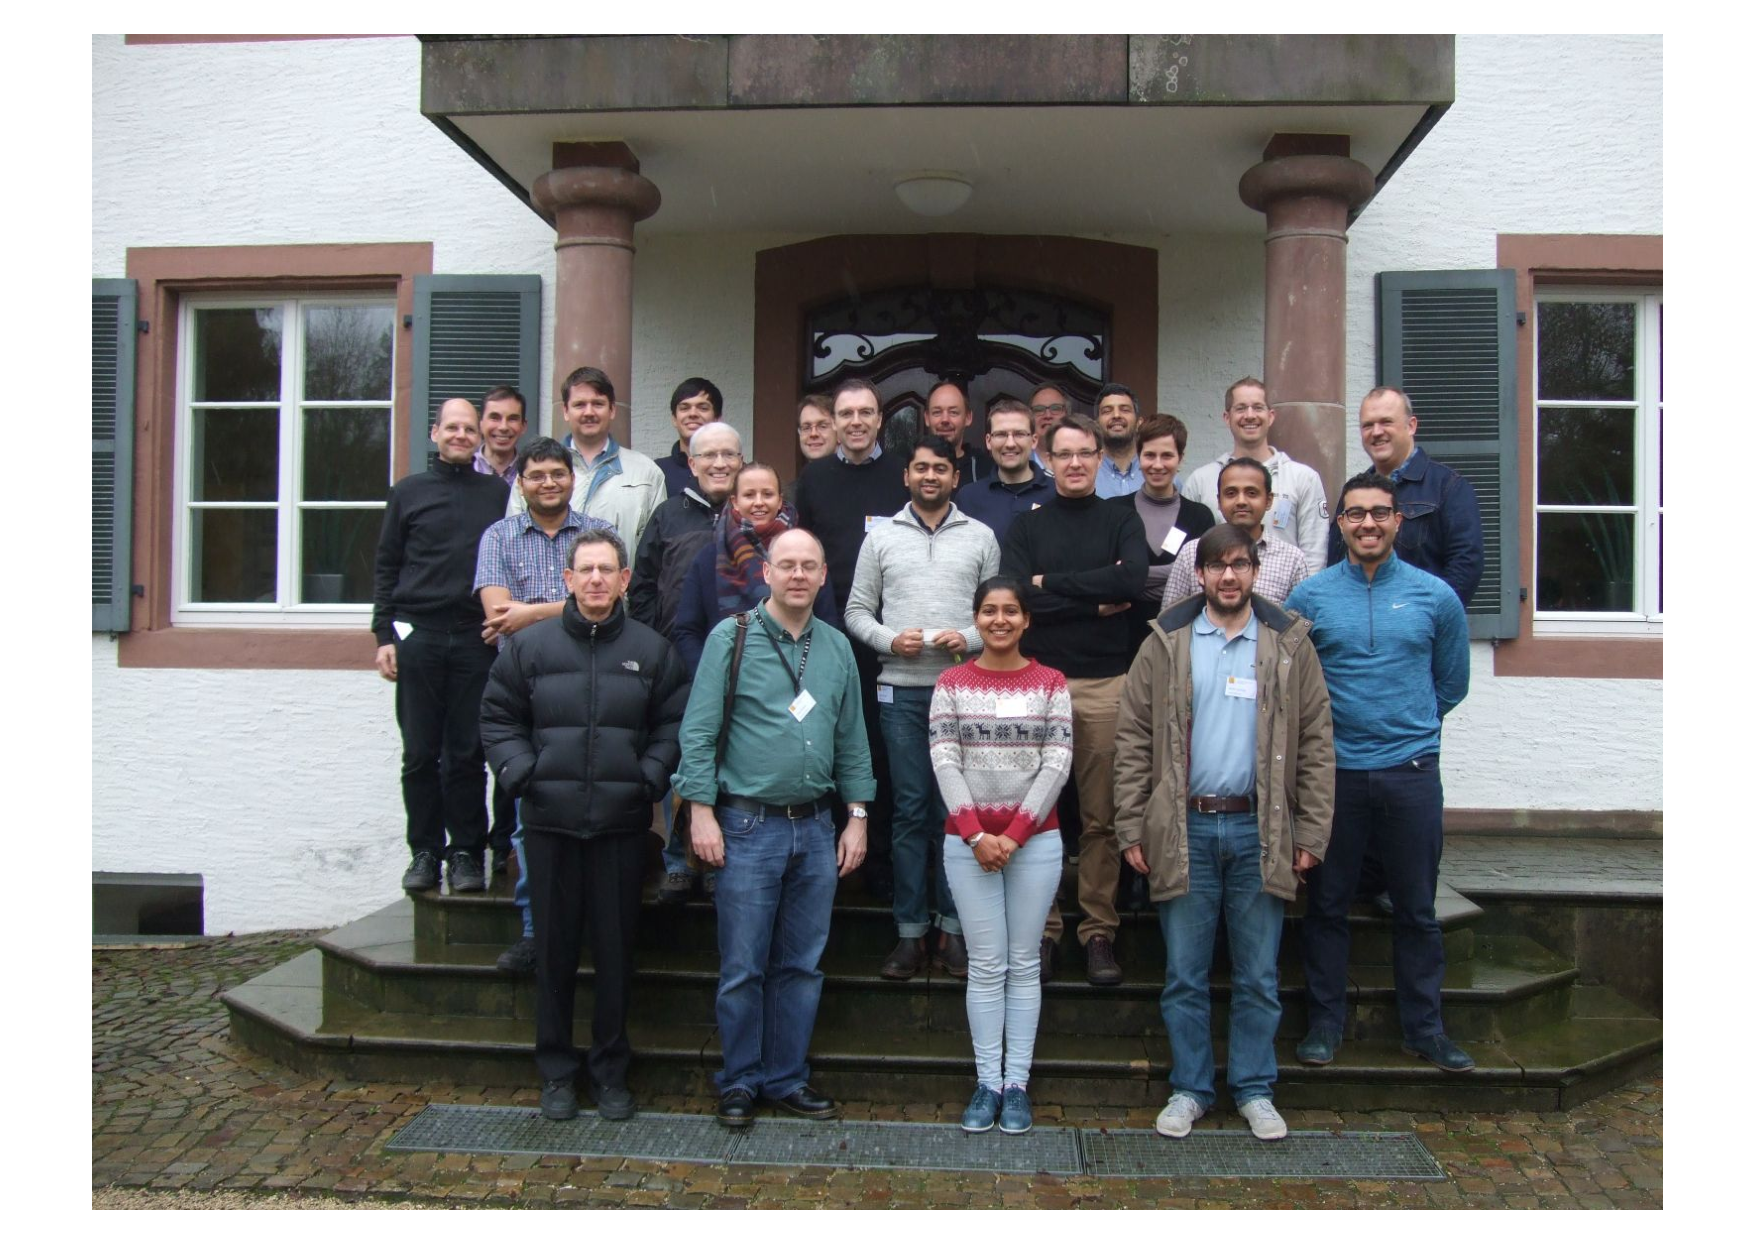
\includegraphics[width=1.0\linewidth]{figures/group-photo}
\end{figure}


%----------------------------------------------------------------------

% bibliography
%----------------------------------------------------------------------
\bibliographystyle{abbrv}

\begin{thebibliography}{10}

\bibitem{dagstuhl-materials}
{Dagstuhl Seminar \#16012 – Global Measurements: Practice and Experience:
  Materials}.
\newblock \url{http://materials.dagstuhl.de/index.php?semnr=16012}.
\newblock [Online; accessed 18-January-2016].

\bibitem{flamingo}
{Flamingo - Management of the Future Internet}.
\newblock \url{http://www.fp7-flamingo.eu}.
\newblock [Online; accessed 18-January-2016].

\bibitem{leone}
{Leone - From Global Measurements to Local Management}.
\newblock \url{http://www.leone-project.eu}.
\newblock [Online; accessed 18-January-2016].

\bibitem{mami}
{MAMI - Measurement and Architecture for a Middleboxed Internet}.
\newblock \url{https://mami-project.eu}.
\newblock [Online; accessed 18-January-2016].

\bibitem{mba}
{Measuring Broadband America - Federal Communications Commission}.
\newblock \url{https://www.fcc.gov/general/measuring-broadband-america}.
\newblock [Online; accessed 18-January-2016].

\bibitem{soti}
{State of the Internet - Akamai}.
\newblock \url{https://www.stateoftheinternet.com}.
\newblock [Online; accessed 18-January-2016].

\bibitem{ethics}
{Workshop on Ethics in Networked Systems Research - ACM SIGCOMM 2015}.
\newblock \url{http://conferences.sigcomm.org/sigcomm/2015/netethics.php}.
\newblock [Online; accessed 18-January-2016].

\bibitem{ripencc:ipj:2015}
{RIPE Atlas: A Global Internet Measurement Network}.
\newblock {\em Internet Protocol Journal}, Sept. 2015.

\bibitem{mallman:imc:2007}
M.~Allman and V.~Paxson.
\newblock {Issues and Etiquette Concerning Use of Shared Measurement Data}.
\newblock IMC '07, pages 135--140. ACM, 2007.

\bibitem{anonymous:ccr:2012}
Anonymous.
\newblock {The Collateral Damage of Internet Censorship by DNS Injection}.
\newblock {\em SIGCOMM Comput. Commun. Rev.}, 42(3):21--27, June 2012.

\bibitem{vbajpai:ccr:2015}
V.~Bajpai, S.~J. Eravuchira, and J.~Sch\"{o}nw\"{a}lder.
\newblock {Lessons Learned From Using the RIPE Atlas Platform for Measurement
  Research}.
\newblock {\em SIGCOMM Comput. Commun. Rev.}, 45(3):35--42, July 2015.

\bibitem{vbajpai:comst:2015}
V.~Bajpai and J.~Sch\"onw\"alder.
\newblock {A Survey on Internet Performance Measurement Platforms and Related
  Standardization Efforts}.
\newblock {\em Communications Surveys Tutorials, IEEE}, 17(3):1313--1341,
  thirdquarter 2015.

\bibitem{sburnett:sigcomm:2015}
S.~Burnett and N.~Feamster.
\newblock {Encore: Lightweight Measurement of Web Censorship with Cross-Origin
  Requests}.
\newblock SIGCOMM '15. ACM, 2015.

\bibitem{jcappos:sigcse:2009}
J.~Cappos, I.~Beschastnikh, A.~Krishnamurthy, and T.~Anderson.
\newblock {Seattle: A Platform for Educational Cloud Computing}.
\newblock SIGCSE '09. ACM, 2009.

\bibitem{fchen:sigcomm:2015}
F.~Chen, R.~K. Sitaraman, and M.~Torres.
\newblock {End-User Mapping: Next Generation Request Routing for Content
  Delivery}.
\newblock SIGCOMM '15. ACM, 2015.

\bibitem{kclaffy:ccr:2016}
k.~claffy.
\newblock {The 7th Workshop on Active Internet Measurements (AIMS7) Report}.
\newblock {\em SIGCOMM Comput. Commun. Rev.}, 46(1):50--57, Jan. 2016.

\bibitem{jcohen:dagstuhl:2014}
J.~E. Cohen, S.~Dietrich, A.~Pras, L.~D. Zuck, and H.~Mireille.
\newblock {Ethics in Data Sharing (Dagstuhl Seminar 14052)}.
\newblock {\em Dagstuhl Reports}, 4(1):170--183, 2014.

\bibitem{gdetal:imc:2013}
G.~Detal, B.~Hesmans, O.~Bonaventure, Y.~Vanaubel, and B.~Donnet.
\newblock {Revealing Middlebox Interference with Tracebox}.
\newblock IMC '13. ACM, 2013.

\bibitem{roland:creds:2014}
S.~Dietrich, J.~van~der Ham, A.~Pras, R.~van Rijswijk-Deij, D.~Shou,
  A.~Sperotto, A.~van Wynsberghe, and L.~Zuck.
\newblock {Ethics in Data Sharing: developing a model for best practice}.
\newblock CREDS II, 2014.

\bibitem{mdischinger:imc:2007}
M.~Dischinger, A.~Haeberlen, K.~P. Gummadi, and S.~Saroiu.
\newblock {Characterizing Residential Broadband Networks}.
\newblock IMC '07. ACM, 2007.

\bibitem{menloreport}
D.~Dittrich and E.~Kenneally.
\newblock {The Menlo Report: Ethical Principles Guiding Information and
  Communication Technology Research}.
\newblock Technical report, U.S. Department of Homeland Security, 2012.

\bibitem{bstiller:aims:2015}
D.~D{\"{o}}nni, G.~S. Machado, C.~Tsiaras, and B.~Stiller.
\newblock {Schengen Routing: {A} Compliance Analysis}.
\newblock In {\em {AIMS} 2015, Ghent, Belgium, June 22-25, 2015.}, 2015.

\bibitem{cdovrolis:ccr:2010}
C.~Dovrolis, K.~Gummadi, A.~Kuzmanovic, and S.~D. Meinrath.
\newblock {Measurement Lab: Overview and an Invitation to the Research
  Community}.
\newblock {\em SIGCOMM Comput. Commun. Rev.}, 40(3):53--56, June 2010.

\bibitem{peardley:dagstuhl:2013}
P.~Eardley, M.~Mellia, J.~Ott, J.~Sch{\"o}nw{\"a}lder, and H.~Schulzrinne.
\newblock {Global Measurement Framework (Dagstuhl Seminar 13472)}.
\newblock {\em Dagstuhl Reports}, 2014.

\bibitem{rfc7594}
P.~Eardley, A.~Morton, M.~Bagnulo, T.~Burbridge, P.~Aitken, and A.~Akhter.
\newblock {A Framework for Large-Scale Measurement of Broadband Performance
  (LMAP)}.
\newblock RFC 7594 (Informational), Sept. 2015.

\bibitem{gcarle:imc:2015}
P.~Emmerich, S.~Gallenm\"{u}ller, D.~Raumer, F.~Wohlfart, and G.~Carle.
\newblock {MoonGen: A Scriptable High-Speed Packet Generator}.
\newblock IMC '15. ACM, 2015.

\bibitem{draft-tsvwg-quic-protocol}
R.~Hamilton, J.~Iyengar, I.~Swett, and A.~Wilk.
\newblock {QUIC: A UDP-Based Secure and Reliable Transport for HTTP/2}.
\newblock Internet-Draft draft-tsvwg-quic-protocol-02, Internet Engineering
  Task Force, Jan. 2016.

\bibitem{mhonda:imc:2011}
M.~Honda, Y.~Nishida, C.~Raiciu, A.~Greenhalgh, M.~Handley, and H.~Tokuda.
\newblock {Is It Still Possible to Extend TCP?}
\newblock IMC '11. ACM, 2011.

\bibitem{pgill:comcom:2011}
B.~Krishnamurthy, W.~Willinger, P.~Gill, and M.~Arlitt.
\newblock {A Socratic method for validation of measurement-based networking
  research}.
\newblock {\em Computer Communications}, 34(1):43 -- 53, 2011.

\bibitem{skrishnan:imc:2012}
S.~S. Krishnan and R.~K. Sitaraman.
\newblock {Video Stream Quality Impacts Viewer Behavior: Inferring Causality
  Using Quasi-experimental Designs}.
\newblock IMC '12, 2012.

\vfill\eject

\bibitem{mluckie:imc:2010}
M.~Luckie.
\newblock {Scamper: A Scalable and Extensible Packet Prober for Active
  Measurement of the Internet}.
\newblock IMC '10. ACM, 2010.

\bibitem{mfiedler:commantel:2013}
T.~N. Minhas and M.~Fiedler.
\newblock {Quality of experience hourglass model}.
\newblock In {\em ComManTel 2013}, Jan 2013.

\bibitem{draft-ietf-ippm-active-passive}
A.~Morton.
\newblock {Active and Passive Metrics and Methods (and everything in-between,
  or Hybrid)}.
\newblock Internet-Draft draft-ietf-ippm-active-passive-06, Internet
  Engineering Task Force, Jan. 2016.

\bibitem{hnam:infocom:2016}
H.~Nam, K.-H. Kim, and H.~Schulzrinne.
\newblock {QoE Matters More Than QoS: Why People Stop Watching Cat Videos}.
\newblock In {\em INFOCOM, 2016 (to appear)}, April 2016.

\bibitem{apathak:pam:2010}
A.~Pathak, Y.~A. Wang, C.~Huang, A.~Greenberg, Y.~C. Hu, R.~Kern, J.~Li, and
  K.~W. Ross.
\newblock {Measuring and Evaluating TCP Splitting for Cloud Services}.
\newblock PAM'10, pages 41--50. Springer-Verlag, 2010.

\bibitem{vpaxson:imc:2004}
V.~Paxson.
\newblock {Strategies for Sound Internet Measurement}.
\newblock IMC '04, pages 263--271. ACM, 2004.

\bibitem{ssundaresan:arxiv:2015}
A.~Razaghpanah, N.~Vallina{-}Rodriguez, S.~Sundaresan, C.~Kreibich, P.~Gill,
  M.~Allman, and V.~Paxson.
\newblock {Haystack: In Situ Mobile Traffic Analysis in User Space}.
\newblock {\em CoRR}, abs/1510.01419, 2015.

\bibitem{rteixeira:pam:2012}
A.~Reggani, F.~Schneider, and R.~Teixeira.
\newblock {An End-Host View on Local Traffic at Home and Work}.
\newblock {PAM} '12, pages 21--31, 2012.

\bibitem{rbush:jsac:2011}
M.~Roughan, W.~Willinger, O.~Maennel, D.~Perouli, and R.~Bush.
\newblock {10 Lessons from 10 Years of Measuring and Modeling the Internet's
  Autonomous Systems}.
\newblock {\em JSAC}, 29(9):1810--1821, October 2011.

\bibitem{gcarle:tma:2015}
J.~Schlamp, R.~Holz, O.~Gasser, A.~Korsten, Q.~Jacquemart, G.~Carle, and E.~W.
  Biersack.
\newblock {Investigating the Nature of Routing Anomalies: Closing in on
  Subprefix Hijacking Attacks}.
\newblock {TMA} '15.

\bibitem{rsitaraman:wiley:2014}
R.~K. Sitaraman, M.~Kasbekar, W.~Lichtenstein, and M.~Jain.
\newblock {\em {Overlay Networks: An Akamai Perspective}}, pages 305--328.
\newblock John Wiley \& Sons, Inc., 2014.

\bibitem{ssonntag:wiopt:2013}
S.~Sonntag, J.~Manner, and L.~Schulte.
\newblock {Netradar - Measuring the wireless world}.
\newblock WiOpt '13, May 2013.

\bibitem{ssundaresan:usenix:2014}
S.~Sundaresan, S.~Burnett, N.~Feamster, and W.~De~Donato.
\newblock {BISmark: A Testbed for Deploying Measurements and Applications in
  Broadband Access Networks}.
\newblock USENIX ATC'14, pages 383--394, 2014.

\bibitem{ssundaresan:pam:2015}
S.~Sundaresan, N.~Feamster, and R.~Teixeira.
\newblock {Measuring the Performance of User Traffic in Home Wireless
  Networks}.
\newblock {PAM} '15, pages 305--317, 2015.

\bibitem{btrammell:commag:2014}
B.~Trammell, P.~Casas, D.~Rossi, A.~Bar, Z.~Houidi, I.~Leontiadis, T.~Szemethy,
  and M.~Mellia.
\newblock {mPlane: an Intelligent Measurement Plane for the Internet}.
\newblock {\em IEEE Communications Magazine}, 52(5):148--156, May 2014.

\bibitem{roland:tnc:2015}
R.~van Rijswijk-Deij.
\newblock {Ethics in Data Sharing: a best practice for NRENs}.
\newblock TNC '15. G\'{E}ANT, 2015.

\bibitem{roland:sigcomm:2015}
R.~van Rijswijk-Deij, M.~Jonker, A.~Sperotto, and A.~Pras.
\newblock {The Internet of Names: A DNS Big Dataset}.
\newblock SIGCOMM '15, pages 91--92. ACM, 2015.

\bibitem{twhite:oreilly:2015}
T.~White.
\newblock {\em {Hadoop - The Definitive Guide: Storage and Analysis at Internet
  Scale {(4.} ed., revised {\&} updated)}}.
\newblock O'Reilly, 2015.

\end{thebibliography}

%----------------------------------------------------------------------

\end{document}
